\documentclass[a4paper]{report}
\usepackage[utf8]{inputenc}
\usepackage[T1]{fontenc}
\usepackage{RJournal}
\usepackage{amsmath,amssymb,array}
\usepackage{booktabs}


% tightlist command for lists without linebreak
\providecommand{\tightlist}{%
  \setlength{\itemsep}{0pt}\setlength{\parskip}{0pt}}

\usepackage{longtable}

% Always define CSL refs as bib entries are contained in separate doc
% Pandoc citation processing
\newlength{\cslhangindent}
\setlength{\cslhangindent}{1.5em}
\newlength{\csllabelwidth}
\setlength{\csllabelwidth}{3em}
\newlength{\cslentryspacingunit} % times entry-spacing
\setlength{\cslentryspacingunit}{\parskip}
% for Pandoc 2.8 to 2.10.1
\newenvironment{cslreferences}%
  {}%
  {\par}
% For Pandoc 2.11+
\newenvironment{CSLReferences}[2] % #1 hanging-ident, #2 entry spacing
 {% don't indent paragraphs
  \setlength{\parindent}{0pt}
  % turn on hanging indent if param 1 is 1
  \ifodd #1
  \let\oldpar\par
  \def\par{\hangindent=\cslhangindent\oldpar}
  \fi
  % set entry spacing
  \setlength{\parskip}{#2\cslentryspacingunit}
 }%
 {}
\usepackage{calc}
\newcommand{\CSLBlock}[1]{#1\hfill\break}
\newcommand{\CSLLeftMargin}[1]{\parbox[t]{\csllabelwidth}{#1}}
\newcommand{\CSLRightInline}[1]{\parbox[t]{\linewidth - \csllabelwidth}{#1}\break}
\newcommand{\CSLIndent}[1]{\hspace{\cslhangindent}#1}



\begin{document}


%% do not edit, for illustration only
\sectionhead{Contributed research article}
\volume{15}
\volnumber{2}
\year{2023}
\month{June}
\setcounter{page}{294}

\begin{article}
  % !TeX root = RJwrapper.tex
\title{genpathmox: An R Package to Tackle Numerous Categorical Variables and Heterogeneity in Partial Least Squares Structural Equation Modeling}


\author{by Giuseppe Lamberti,}

\maketitle

\abstract{%
Partial least squares structural equation modeling (PLS-SEM), combined with the analysis of the effects of categorical variables after estimating the model, is a well-established statistical approach to the study of complex relationships between variables. However, the statistical methods and software packages available are limited when we are interested in assessing the effects of several categorical variables and shaping different groups following different models. Following the framework established by Lamberti, Aluja, and Sanchez (2016), we have developed the ~\href{https://CRAN.R-project.org/package=genpathmox}{genpathmox} \emph{R} package~for~handling a large number of categorical variables when faced with heterogeneity in PLS-SEM. The package has functions for various aspects of the analysis of heterogeneity in~PLS-SEM models,~including estimation, visualization, and hypothesis testing. In this paper, we describe the implementation of~genpathmox~in detail and demonstrate its usefulness by analyzing employee satisfaction data.
}

\hypertarget{introduction}{%
\section{Introduction}\label{introduction}}

Partial least squares structural equation modeling (PLS-SEM; (Wold 1985))
is a method for estimating causal relationships between observed
variables and hypothesized latent variables (Evermann and Rönkkö 2021). PLS-SEM was
developed initially as an alternative to the classical covariance
based-structural equation modeling (CB-SEM) that estimates latent
variables (LVs) as~common factors that explain co-variation between the
associated indicators (Hair Jr, Matthews, et al. 2017).~However, in the last fifteen years it
has become a reference for estimating causal models, in particular in
marketing and management research
(Becker et al. 2022; Sarstedt, Hair, et al. 2022; Sarstedt, Hair Jr, and Ringle 2022; Hair Jr et al. 2021; Henseler 2020; Evermann and Rönkkö 2021).

Concurrent with the affirmation of the PLS-SEM approach for estimating
causal models, there has been a corresponding surge in research
addressing the issue of heterogeneity in parameter estimation.This
arises when the existence of different models is assumed for data
characterized by differences in the coefficients that explain causal
relationships between LVs. In this scenario, a single model could
provide a biased view of those causal relationships. ~The literature
describes several approaches to tackling heterogeneity that can be
classified in terms of~observed heterogeneity, and non-observed
heterogeneity (for a detailed review of the PLS-SEM analysis in the
presence of heterogeneity, see (Klesel et al. 2022))

Observed heterogeneity is based on the hypothesis that the underlying
relationship between latent variables vary by certain categorical
variables (CVs), for example sociodemographic factors such as gender,
education, or social status, such that the data can be separated into
groups and a different model can be fit to each group. The presence of
observed heterogeneity is then verified by testing whether the
coefficients of the estimated models are significantly different between
groups (Hair Jr, Sarstedt, et al. 2017). Belonging to this category are the classical PLS
multigroup tests, including the parametric (Keil et al. 2000), permutation
(Chin and Dibbern 2010), and Henseler (Henseler, Ringle, and Sinkovics 2009) tests, as well as the more recent
approach proposed by Klesel et al. (2019). As for non-observed heterogeneity, this
is present when differences are inherent to the data. In this scenario,
a different approach is required, and different models are typically
identified following a latent class analysis (Sarstedt, Radomir, et al. 2022)~or
clustering (Esposito Vinzi et al. 2008) approach.

Methodological advances and the increase in applications have led to the
development of numerous \emph{R} packages, starting with
\href{https://CRAN.R-project.org/package=plspm}{plspm} (Sanchez, Trinchera, and Russolillo 2015), subsequently
followed by \href{https://CRAN.R-project.org/package=cSEM}{cSEM} (Rademaker and Schuberth 2020) and
\href{https://CRAN.R-project.org/package=SEMinR}{SEMinR} (Ray, Danks, and Valdez 2020), both of
which incorporate recent developments in the PLS approach, including
improved estimation (consistent PLS (PLSc) (Dijkstra and Henseler 2015)), improved
validation criteria (the PLSpredict approach to prediction
(Shmueli et al. 2016, 2019)), new reliability measures
(Dijkstra and Henseler 2015; Hair Jr et al. 2019), and also
\href{https://CRAN.R-project.org/package=matrixpls}{matrixpls} (Rönkkö 2017),
particularly used for simulation studies. Concerning heterogeneity, the
cSEM package allows multigroup analysis with several embedded tests.~
Pathmox analysis (Sanchez and Aluja 2006; Lamberti, Aluja, and Sanchez 2016; Lamberti, Banet Aluja, and Sanchez 2017) was proposed as
a useful method when observed heterogeneity is assumed, but several
potential CVs exist that could define different groups and models. This
method explores and identifies, using an iterative algorithm, the most
significantly different groups associated with significant differences
in models. The algorithm follows a segmentation tree approach, where
each node is a PLS-SEM model. Differences are compared and partitions
are chosen that define the most significant divergences between
coefficients (Lamberti, Aluja, and Sanchez 2016). ~The algorithm has been further improved,
first by including a statistical test capable of identifying, for each
split, the model coefficient responsible for the partitions
(Lamberti, Banet Aluja, and Sanchez 2017), and then by combining the pathmox algorithm with
classical multigroup analysis in a new approach called hybrid multigroup
analysis ~(Lamberti 2021).~

In this paper, we describe the
\href{https://CRAN.R-project.org/package=genpathmox}{genpathmox} package
(Lamberti 2022) which implements the classical pathmox analysis and the
more recently developed hybrid multigroup analysis (Lamberti 2021). The
package, initially developed in 2014, has been updated to include recent
methodological advances (including PLSc; (Dijkstra and Henseler 2015)) and has also
been modified to work jointly with the cSEM package to increase
analytical flexibility.~Below we first review the framework formalized
by~Lamberti, Aluja, and Sanchez (2016), then provide an overview of the genpathmox package, and
finally, we demonstrate the use of the package on real-world analysis of
employee satisfaction data and work climate drivers.

\hypertarget{overview-of-the-pathmox-methodology}{%
\section{Overview of the pathmox methodology}\label{overview-of-the-pathmox-methodology}}

Pathmox analysis (Lamberti, Aluja, and Sanchez 2016; Lamberti, Banet Aluja, and Sanchez 2017) was introduced to handle
observed heterogeneity in PLS-SEM when several CVs are present. ~Unlike
classical methods for tackling observed heterogeneity in PLS-SEM,
instead of testing whether a CV produces a significant difference in
model coefficients (i.e., a confirmatory approach), an exploratory
approach is adopted. That is, the aim of pathmox is to identify
siginificantly different groups associated with different PLS models,
provided they exist. The algorithm applies a binary tree partitioning
approach. It first estimates a single global model for the entire
dataset to define the root node of the tree, and then explores all
possible binary partitions for each CV. Differences in coefficients are
statistically evaluated by the \(F\)-global test (Lamberti, Aluja, and Sanchez 2016). This test
provides a global measure of the degree of difference between partitions
(i.e., a \(p\)-value). ~Comparisons are then sorted in descending order
based on the \(p\)-values, and the partition with the smallest \(p\)-value
(i.e.~one which suggests the greatest difference from the root model) is
then chosen as optimal.~

The degree of difference between models (the split criterion) is
determined by applying a test, inspired by ~Chow (1960) and Lebart, Morineau, and Fenelon (1979) which
compares differences between the coefficients of two linear regression
models. In pathmox, the difference between two PLS-SEM models is
determined by comparing structural model coefficients, i.e., by
comparing, as in the case of Chow (1960) and Lebart, Morineau, and Fenelon (1979), restricted deviance
vs.~unrestricted deviance, defined, respectively, as the deviance
calculated for the whole sample considering a single model valid for all
the observations, and the sum of the model deviances estimated for each
group of observations. ~

From a graphical standpoint, pathmox is not much different from a
classical segmentation tree -- as the algorithm produces a tree with a
root, intermediate nodes, and terminal nodes -- other than that each
node is associated with a PLS model.~

\hypertarget{the-split-criterion}{%
\subsection{The split criterion}\label{the-split-criterion}}

The split criterion used to define the tree partitions is a critical
aspect of the pathmox algorithm. Below we describe the \(F\)-global test,
the formulation of the null and alternative hypotheses, and the
statistic used to test the null hypothesis (further details are
available in (Lamberti, Aluja, and Sanchez 2016)).

Consider a simple structural model with one dependent LV, denoted by the
Greek letter \textbf{\(\eta\)}, and explained by a generic set of independent
LVs denoted by the matrix ~\textbf{X} = \(\{\xi_{ip}\}\), where
\(i = 1, \ldots, n\) refers to the observation, and where
\(p = 1, \ldots, P\) refers to the LV. Its generalization into a more
complex model is straightforward.~

Using the matrix form, the model can be expressed as:~ \[\label{eq1}
\boldsymbol{\eta} = \textbf{X}\boldsymbol{\beta} + \boldsymbol{\varepsilon}\]
where \(\boldsymbol{\beta}\) is the vector of the regression coefficients
of \(\boldsymbol{\eta}\), and where \(\boldsymbol{\varepsilon}\) is the
disturbance term. Let the data ~be partitioned by rows, where the
partition is determined by a CV ~with ~\emph{m} categories (i.e., segments or
groups). The number of units in group \emph{g} (\(g=1,\ldots, m\)) is denoted
by \(n_g\), and ~the total sample size can be expressed as
\(n=\sum_{g=1}^m n_g\). The \(F\)-global test compares model coefficients
only by considering binary partitions. This means that the number of
comparisons depends on the nature of the CVs. With a dummy (binary) CV,
there is just a single comparison. With a nominal CV, there are
\(2^{m-1}-1\) comparisons. Finally, with an ordinal CV, there are \(m-1\)
comparisons.

The logic of ~the test is to compare the coefficients of two models,
while considering two different scenarios. Under the null hypothesis, we
assume that one model is valid for all observations. This implies that
one coefficient for each independent LV is enough to explain the
dependent LV. If we consider the simplest case of a dummy CV (\emph{m}=2),
denoting the two groups as \(A\) and \(B\), the null and alternative
hypotheses can be formulated as:

\[\begin{aligned}
\label{eq2}
H_0: \boldsymbol{\beta}_A = \boldsymbol{\beta}_B \\
H_1: \boldsymbol{\beta}_A \ne \boldsymbol{\beta}_B
\end{aligned}\] According to the null and alternative hypotheses, and
following Lebart, Morineau, and Fenelon (1979), we can rearrange Eq.
\protect\hyperlink{eq1}{\[eq1\]} as follows:

\[\label{eq22}
\left[\begin{array}{l}
\boldsymbol{\eta}_A \\
\boldsymbol{\eta}_B 
\end{array}\right] \quad
\left[\begin{array}{l}
\textbf{X}_A \\
\textbf{X}_B 
\end{array}\right] \quad
\left[\begin{array}{l}
\boldsymbol{\beta}
\end{array}\right]  \quad +
\left[\begin{array}{l}
\boldsymbol{\varepsilon}_A \\
\boldsymbol{\varepsilon}_B 
\end{array}\right]\]

\[\label{eq23}
\left[\begin{array}{l}
\boldsymbol{\eta}_A \\
\boldsymbol{\eta}_B 
\end{array}\right] \quad
\left[\begin{array}{cc}
\textbf{X}_A \quad0\\
0 \quad\textbf{X}_B 
\end{array}\right] \quad
\left[\begin{array}{l}
\boldsymbol{\beta}_A \\
\boldsymbol{\beta}_B
\end{array}\right]  \quad +
\left[\begin{array}{l}
\boldsymbol{\varepsilon}_A \\
\boldsymbol{\varepsilon}_B 
\end{array}\right]\]

We calculate the deviance (the sum of squared residuals, SSR) for both
models: \(SSR_{H0}\) under the null hypothesis and \(SSR_{H1}\) under the
alternative. Finally, we test the null hypothesis using the following
statistic:

\[\label{F_global}
F  = \frac{\left(SSR_{H_0}-SSR_{H_1}\right) \Bigg/p}{SSR_{H_1}\Bigg/n-2p}\]
which follows an \(F\) distribution with \(p\) and \(\left(n - 2p\right)\)
degrees of freedom, where \(p\) is the number of explanatory LVs, and
where \(n = n_A + n_B\) is the total number of observations.

\hypertarget{improving-tree-partition-interpretation-the-f-coefficient-test}{%
\subsection{\texorpdfstring{Improving tree partition interpretation: the \(F\)-coefficient test}{Improving tree partition interpretation: the F-coefficient test}}\label{improving-tree-partition-interpretation-the-f-coefficient-test}}

The \(F\)-coefficient test was an important improvement in the algorithm
introduced in Lamberti, Banet Aluja, and Sanchez (2017). The \(F\)-global test used in pathmox as a
split criterion is a global criterion that establishes whether or not
the CV reflects a significant difference. However, it does not provide
information as to which coefficients are responsible for that
difference. ~The \(F\)-coefficient test~complements the split criterion in
pathmox by providing information about which coefficients may be
responsible for the significant difference.

Rearranging the model formulated by Eq.
\protect\hyperlink{eq1}{\[eq1\]}, we consider the
particular case of one dependent LV denoted \(\eta\), and two predictor
LVs denoted \(\xi_1\) and \(\xi_2\):

\[\label{eq4}
\boldsymbol{\eta} = \boldsymbol{\xi}_1\beta_1 + \boldsymbol{\xi}_2\beta_2 + \boldsymbol{\varepsilon}\]

Let us assume that a significant difference exists between the models
estimated for the two groups, \(A\) and \(B\), as defined by a generic dummy
variable. Applying the \(F\)-global test (Lamberti, Aluja, and Sanchez 2016) we cannot determine
whether the difference between the two models depends on \(\xi_1\) or
\(\xi_2\), or depends on both. However the null hypotheses for \(\beta_1\)
and \(\beta_2\), and the corresponding alternative hypotheses, can be
reformulated to determine whether the coefficients estimated for the
predictors are significantly different, as follows:\footnote{Note that the alternative hypothesis is the same for both \(\xi_1\)
  and \(\xi_2\).}
\[\begin{aligned}
\label{eq5}
H_0: &\beta_{iA} =\beta_{iB}  \quad  \text{with i }= 1, 2\\
H_1: &\boldsymbol{\beta}_A \ne \boldsymbol{\beta}_B
\end{aligned}\] According to the null and alternative hypotheses, and
following Lebart, Morineau, and Fenelon (1979), we can rearrange Eqs.
\protect\hyperlink{eq22}{\[eq22\]} and
\protect\hyperlink{eq23}{\[eq23\]} as:

\[\label{nul2}
\left[\begin{array}{l}
\boldsymbol{\eta}_A \\
\boldsymbol{\eta}_B 
\end{array}\right] \quad
\left[\begin{array}{ccc}
\boldsymbol{\xi}_{1A}\quad 0 \quad0\\
0 \quad\boldsymbol{\xi}_{2A} \quad0\\
\boldsymbol{\xi}_{1B} \quad0 \quad0\\
0 \quad0 \quad\boldsymbol{\xi}_{2B}\\
\end{array}\right] \quad
\left[\begin{array}{l}
\beta_1 \\
\beta_{2A} \\
\beta_{2A} \\
\end{array}\right]  \quad +
\left[\begin{array}{l}
\boldsymbol{\varepsilon}_A \\
\boldsymbol{\varepsilon}_B 
\end{array}\right]\]

\[\label{nul22}
\left[\begin{array}{l}
\boldsymbol{\eta}_A \\
\boldsymbol{\eta}_B 
\end{array}\right] \quad
\left[\begin{array}{ccc}
\boldsymbol{\xi}_{1A}\quad 0 \quad0\\
0 \quad\boldsymbol{\xi}_{2A} \quad0\\
0 \quad0 \quad\boldsymbol{\xi}_{1B}\\
0 \quad\boldsymbol{\xi}_{2B} \quad0\\
\end{array}\right] \quad
\left[\begin{array}{l}
\beta_{1A} \\
\beta_{1B} \\
\beta_2 \\
\end{array}\right]  \quad +
\left[\begin{array}{l}
\boldsymbol{\varepsilon}_A \\
\boldsymbol{\varepsilon}_B 
\end{array}\right]\]

\[\label{al2}
\left[\begin{array}{l}
\boldsymbol{\eta}_A \\
\boldsymbol{\eta}_B 
\end{array}\right] \quad
\left[\begin{array}{ccc}
\boldsymbol{\xi}_{1A}\quad 0 \quad0 \quad0\\
0 \quad\boldsymbol{\xi}_{2A}\quad0 \quad0\\
0 \quad0 \quad\boldsymbol{\xi}_{1B} \quad0\\
0 \quad0 \quad0 \quad \boldsymbol{\xi}_{2B}\\
\end{array}\right] \quad
\left[\begin{array}{l}
\beta_{1A} \\
\beta_{1B} \\
\beta_{2A} \\
\beta_{2B} \\
\end{array}\right]  \quad +
\left[\begin{array}{l}
\boldsymbol{\varepsilon}_A \\
\boldsymbol{\varepsilon}_B 
\end{array}\right]\]

We calculate again the deviance for both models (\(SSR_{H0}\) and
\(SSR_{H1}\)) and test the null hypothesis using the following statistic:

\[\label{F_coefl}
F_i  = \frac{\left(SSR_{H_{0_{\beta_i}}}-SSR_{H_1}\right) \Bigg/1}{SSR_{H_1}\Bigg/2\left(n-\sum p\right)}  \; \text{with i=1,2}\]
which follows an \(F\) distribution with \(1\) and
\(2\left(n - \sum p\right)\) degrees of freedom, and where \(p\) is the
number of explanatory LVs, and \(n = n_A + n_B\) is the total number of
observations.

Note that both the \(F\)-global and the \(F\)-coefficient are implemented in
the genpathmox package.

\hypertarget{stop-criteria}{%
\subsection{Stop criteria}\label{stop-criteria}}

Since pathmox is an iterative algorithm, its convergence depends on the
specific stop criteria adopted by the user. Three criteria (all
implemented in the genpathmox package) are proposed in Lamberti, Aluja, and Sanchez (2016):

\begin{enumerate}
\def\labelenumi{\arabic{enumi}.}
\item
  A more significant partition is not found. This means that the null
  hypothesis is not rejected in any of the candidate partitions, and
  as the obtained models are similar to each other, it makes no sense
  to continue splitting the data. This condition is also strictly
  related to the significance threshold of the \(p\)-value chosen by the
  user, usually set to 0.05 (a typical \(p\)-value threshold in PLS-SEM
  applications).
\item
  Maximum tree depth is achieved. This is related to the number of
  terminal nodes required by the user, a choice based on the
  complexity of the model and the number of CVs used. Generally
  speaking, trees of 2-3 levels (with a maximum of 4-8 associated
  terminal nodes) are preferred.\footnote{A greater tree depth results in a higher number of terminal nodes,
    with the direct consequence of having to make more comparisons
    between model coefficients, and with results that may not always be
    easy to interpret.}
\item
  A node has too few observations to be partitioned. PLS-SEM works
  well with a relatively small number of observations, but it is
  recommended to fix a threshold of a relatively large number of
  observations to ensure that nodes are representative. For
  exploratory purposes, the recommended number of observations in each
  node is between 50 and 100. ~
\end{enumerate}

\hypertarget{pathmox-to-reduce-the-number-of-comparisons-before-running-multigroup-analysis-hybrid-multigroup-analysis}{%
\subsection{Pathmox to reduce the number of comparisons before running multigroup analysis: hybrid multigroup analysis}\label{pathmox-to-reduce-the-number-of-comparisons-before-running-multigroup-analysis-hybrid-multigroup-analysis}}

A criticism of the multigroup approach is that differences between
coefficients could be difficult to interpret when the number of
comparisons is high. This could happen when we have to simultaneously
analyze more than one CV, or when the CV has more than 3 or 4 levels.

The pathmox algorithm does not perform an a posteriori statistical
comparison of the coefficients of the models associated with the
terminal nodes, nor does it establish the invariance between groups that
is an important aspect of comparing PLS-SEM models (Henseler, Ringle, and Sarstedt 2016).\footnote{Invariance ensures that a dissimilar group-specific model estimate
  does not depend on diverse LV meaning across groups. A specific
  procedure to verify measurement invariance in the PLS-PM framework
  -- proposed by Henseler, Ringle, and Sarstedt (2016) -- is measurement invariance of composite
  models (MICOM), consisting of three hierarchical steps: (1)
  configural invariance, which ensures the same LV specifications when
  LVs are equally parameterized and estimated across groups, (2)
  compositional invariance, which ensures that LV scores reflect the
  same construct across groups, and (3) equality of latent variables,
  which means that values and variances ensure that data can be pooled
  across groups. If all three steps are confirmed, full measurement
  invariance is established, while if only the first two steps are
  confirmed partial measurement invariance is established. Step one
  and two are necessary condition for performing multigroup analysis.
  A practical guideline on applying MICOM is provided by (Hair Jr, Sarstedt, et al. 2017),
  while Henseler, Ringle, and Sarstedt (2016) provide more details on methodological aspects.}
However, pathmox can be used just to reduce the number of groups to
compare before running a classical multigroup analysis. Instead of using
the original CV, the multigroup comparison uses a new intersection CV
defined by the CV groups resulting from the tree partitions. This is
called the hybrid segmentation variable (Lamberti 2021), which is used for
the hybrid multigroup analysis.~

The hybrid multigroup analysis consists of sequential steps as follows:

\begin{enumerate}
\def\labelenumi{\arabic{enumi}.}
\item
  Use pathmox to identify the most significantly different groups
\item
  Use multigroup analysis to compare the groups:

  \begin{enumerate}
  \def\labelenumii{\arabic{enumii}.}
  \item
    Test the invariance of the constructs among groups using the
    MICOM procedure (Henseler, Ringle, and Sarstedt 2016)
  \item
    Test the statistical differences between models using a
    criterion proposed by the literature (Klesel et al. 2022).
  \end{enumerate}
\end{enumerate}

Note that the genpathmox package does not include any function to
automatically run the hybrid multigroup analysis. Rather, this analysis
is done, as will be shown below, by combining the genpathmox and cSEM
(using the functions testMICOM() to test invariance, and testMGD() to
compare coefficients).

\hypertarget{pathmox-advantages-and-limitations}{%
\subsection{Pathmox advantages and limitations}\label{pathmox-advantages-and-limitations}}

A first advantage of pathmox is that, given a set of CVs, it yields the
most significantly different groups associated with the most
significantly different models. The algorithm reduces the number of
groups to be compared and analyzed, with the direct consequence that the
user merely has to interpret the differences. A second advantage is that
it ranks CVs by their importance in the split process (as in other
classical tree partitioning procedures). This is important because an
analysis of differences in PLS-SEM with more CVs involves not only
comparing groups, but also establishing the most significant sources of
heterogeneity in defining differences.

The main limitation of pathmox is related to the split criteria. The
fact that the algorithm realizes an exhaustive search over unadjusted
\(p\)-values to determine the best partition could potentially produce
biased results (Loh and Shih 1997). A possible solution would be to apply a
Bonferroni correction for multiple comparisons, but this is not yet
available in the current version of the package.~The \(F\)-global and the
\(F\)-coefficients are parametric tests based on a classical parametric
statistic: the \(F\)-statistic. This supposes the normality assumption of
the perturbation terms with equal variance in all dependent constructs,
even though the assumptions are rarely met in practice. Nevertheless,
the sensitivity of the \(F\)-statistic is guaranteed by a larger sample
size, lower levels of random perturbations, and clearer differences in
the segments, as shown by the simulations performed by Lamberti, Aluja, and Sanchez (2016; Lamberti, Banet Aluja, and Sanchez 2017). Another important limitation is that pathmox focuses only
on the problem of detecting the path coefficients that are responsible
for differences between PLS-SEM models, by adapting the measurement
model to each segment. This leads to the problem of invariance, which
greatly increases in importance when we analyze data with potential
sources of heterogeneity by fitting one model to each segment. In this
situation, it could become difficult to guarantee that each construct in
each segment is measuring the same latent construct.

Finally, it is important to remark that the \(F\)-tests are determined by
the sum of the squares of the residuals of the structural model in
parent and children nodes and using the composite scores. Indeed, in the
case of the common factor, the composites scores can just be used as
common factor proxies since they are contaminated by measurement random
error. Hence, the \(F\)-test ranking of the CVs may not be optimum when
there is a small number of indicators per latent variable. Researchers
who intend to apply pathmox when common factors are present in the model
should take this limitation into account in performing the analysis;
alternatively they should use the classical PLS algorithm modifying the
options of the genpathmox functions accordingly.

\hypertarget{the-genpathmox-package}{%
\section{\texorpdfstring{The \emph{genpathmox} package}{The genpathmox package}}\label{the-genpathmox-package}}

\hypertarget{overview}{%
\subsection{Overview}\label{overview}}

The genpathmox package is based on one main function called
pls.pathmox(), which implements the pathmox algorithm and provides
results for analysis. Four additional functions are a summary()
function, and three plot functions ( plot(), bar\_impvar(),
bar\_terminal()) that help the user to interpret results. In practice,
users should first apply the main function pls.pathmox() to generate a
" plstree" object. The components of this object include tree
partition results, fitted coefficients of the PLS models for each
terminal node, and other results to be used for the analysis. The "
plstree" object plays an instrumental role, as it is a necessary input
for the other functions in the package. This design is convenient, as
details of data, PLS model, and tree split rules need only be specified
once in pls.pathmox(), and are passed to other functions.

The summary() function provides a complete output of all results, plot()
provides the segmentation tree plot, bar\_impvar() provides a bar plot of
the ranking by importance of the CVs that participate in the split
process, and bar\_terminal() produces a bar plot of the coefficients of
the PLS terminal nodes of the tree, enabling intuitive analysis of the
differences between them.

The genpathmox package has been designed to interact with the cSEM
package (Rademaker and Schuberth 2020), one of the latest and most complete packages for
PLS-SEM analysis. This package can be used to analyze each model
associated with the terminal nodes identified by pathmox and to run the
hybrid multigroup analysis. To that end, the " plstree" object also
contains a list of datasets called .hybrid, corresponding to lists of
datasets of observations belonging in the tree terminal nodes.

Using the .hybrid list combined with the cSEM::csem(), each terminal
node can be easily and completely analyzed in terms of model validation,
coefficient estimation, and inference. The resulting object generated by
csem() can then be passed to testMICOM() to verify the invariance of the
model constructs for the terminal nodes, and to testMGD() to compare the
coefficients. The hybrid multigroup approach (Lamberti 2021) can then be
implemented. Further details on how to use the cSEM package are
available in Rademaker and Schuberth (2020).

Figure ~\protect\hyperlink{figure:flow}{1}
illustrates how to use the genpathmox package. On the left, the grey
block contains the input elements, i.e., the data, the model, and the
tree rules. Calling up pls.pathmox() generates the " plstree" object,
as shown in the central orange block, which yields estimation and
visualization results, as shown in the two orange blocks on the right.
Finally, plstree\$hybrid is used as the input parameter of the cSEM
package, yielding full results for the terminal nodes and the multigroup
analysis, as shown in the blue blocks.

\begin{figure}
\hypertarget{figure:flow}{%
\centering
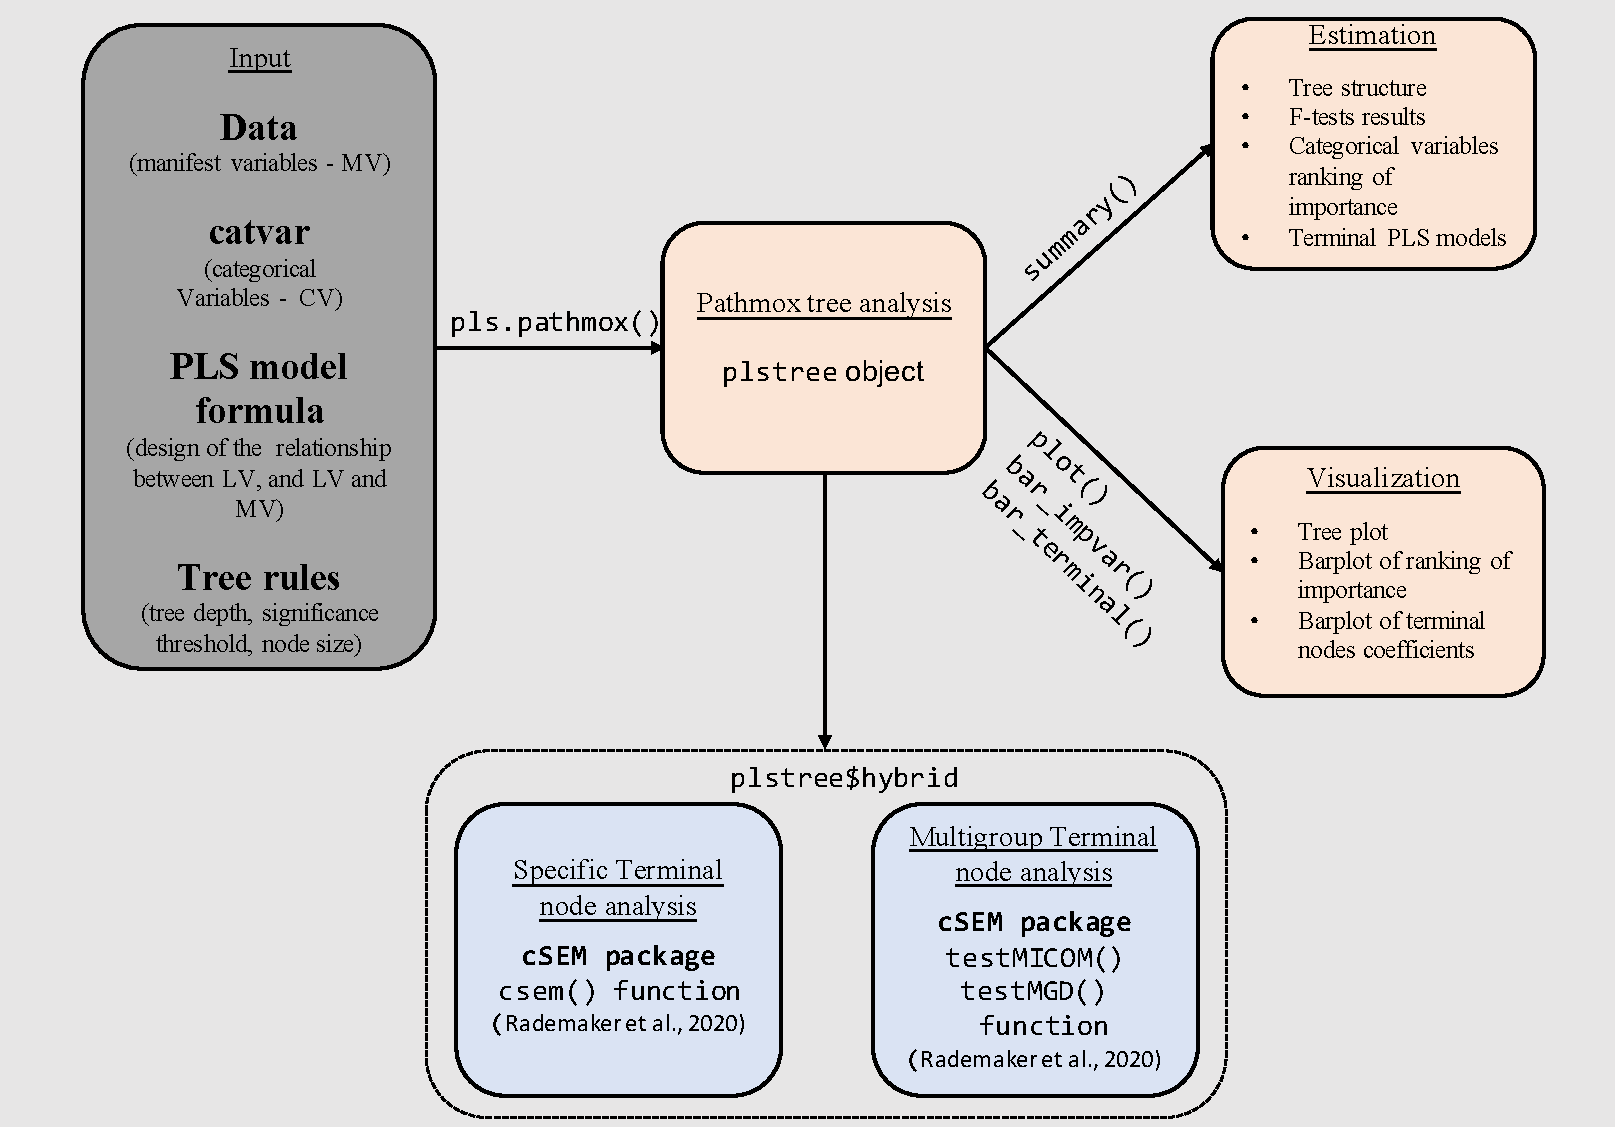
\includegraphics[width=\textwidth,height=8cm]{Fig1_flow.pdf}
\caption{Illustration of genpathmox package
functions}\label{figure:flow}
}
\end{figure}

\hypertarget{implementation-of-main-functions}{%
\subsection{Implementation of main functions}\label{implementation-of-main-functions}}

\hypertarget{estimation-function-pls.pathmox}{%
\subsection{Estimation function: pls.pathmox}\label{estimation-function-pls.pathmox}}

To apply the pls.pathmox function, users need to specify at least three
arguments:

\begin{enumerate}
\def\labelenumi{\arabic{enumi}.}
\item
  .model. A formula specifying the model described using syntax
  inspired by the lavaan package (Rosseel 2012). Structural and measurement
  models are defined by enclosure between double quotes. The
  directional link between constructs is defined using the
  ("\(\sim\)") operator. The dependent LV is on the left-hand side of
  the operator, and the explanatory LVs, separated by the ("+")
  operator, are on the right-hand side. As for the outer model, LVs
  are defined by listing the corresponding indicators after the
  operator ("\(=\sim\)") if the LV is modelled as a common factor, or
  the operator("\(<\sim\)") if the LV is modelled as a composite. On
  the left-hand side of the operator is the LV, and on the right-hand
  side are the indicators separated by the ("+") operator. Please
  note that variable labels cannot contain (".") (for details of the
  meaning of modes A and B, see (Hair Jr et al. 2016)).
\item
  .data. A matrix or data frame containing the indicators.
\item
  .catvar. A single factor or set of factors organized as a data frame
  containing the CVs used as sources of heterogeneity.
\end{enumerate}

Other input parameters have default values. Table
~\protect\hyperlink{par_imp}{1} reports the
meaning of each parameter and the admissible and default values.

\hypertarget{par_imp}{}
\begin{longtable}[]{@{}llll@{}}
\caption{Input parameters with default values}\tabularnewline
\toprule\noalign{}
Parameter & Purpose & Possible values & Default values \\
\midrule\noalign{}
\endfirsthead
\toprule\noalign{}
Parameter & Purpose & Possible values & Default values \\
\midrule\noalign{}
\endhead
\bottomrule\noalign{}
\endlastfoot
.scheme & inner weighting scheme & " centroid", " factorial", or " path" & " path" \\
.consistent & consistent PLS estimation (Dijkstra and Henseler 2015) is used instead of classical approach (Wold 1985) & TRUE or FALSE & TRUE \\
.alpha & minimum threshold significance & values belonging the interval \([0,1]\) & 0.05 \\
.deep & maximum tree depth & an integer \(\geq\) 1 & 2 \\
.size & minimum proportion of total sample admissible for a node size & value belonging the interval \([0,1]\) & 0.10 \\
.candidate size & minimum admissible size for a candidate node & an integer \(\geq\) 0 & 50 \\
.tree & logic parameter to show the tree plot & TRUE or FALSE & TRUE \\
\end{longtable}

Once the split process is complete, results are saved in the object of
class " plstree" , which contains all the results necessary to
interpret the pathmox analysis (see Table
~\protect\hyperlink{output}{2})

\hypertarget{output}{}
\begin{longtable}[]{@{}ll@{}}
\caption{" plstree" results}\tabularnewline
\toprule\noalign{}
Results & Use \\
\midrule\noalign{}
\endfirsthead
\toprule\noalign{}
Results & Use \\
\midrule\noalign{}
\endhead
\bottomrule\noalign{}
\endlastfoot
MOX & provides information on the tree structure: node type (intermediate or terminal), node size, binary split \\
terminal\_paths & allows visualization of path coefficients and \(R^2\) for each terminal node \\
var\_imp & provides a ranking of the CVs used in the split process \\
Fg.r & identifies which CV is responsible for the partition \\
Fc.r & identifies the path coefficient responsible for the partition \\
hybrid & subsets of data associated with each terminal node \\
\end{longtable}

\hypertarget{visualization-functions-plot-bar_impvar-and-bar_terminal}{%
\subsection{Visualization functions: plot, bar\_impvar and bar\_terminal}\label{visualization-functions-plot-bar_impvar-and-bar_terminal}}

Three types of plots are possible in the \textbf{genpathmox} package: a
pathmox treeplot, a barplot which displays the ranking of the CVs, and a
barplot of the PLS-SEM coefficients of the terminal nodes. The tree plot
is obtained by applying the plot() function, which returns a tree
structure with root, intermediate, and terminal nodes. For each
partition, the \(F\)-global test \(p\)-value is reported with the associated
CV, and the number of observations associated with each node. The plot
is implemented using functions from the diagram package (Soetaert 2020). The
plot of the CV ranking is obtained using the bar\_impvar() function. This
function uses the barplot() function to visualize the importance of the
CVs. The importance of each CV is based on the \(F\)-statistic of the
\(F\)-global test calculated for each CV in each tree node. Finally, the
plot of the coefficients of the PLS-SEM model for each terminal node is
obtained using the bar\_terminal() function, also based on the barplot()
function, which allows a more intuitive comparison of the coefficients
of the terminal nodes.

The user can choose between two bar plot visualizations: (1) a plot of
all the coefficients of the same model in the same plot, which is useful
for comparing the terminal nodes models, and (2) a plot of the same
coefficients for all terminal nodes in the same plot (lines correspond
to the coefficients and bars report the coefficient effects), useful for
a more direct comparison of a specific coefficient between models. In
the former, the bar plot depicted for each model also plots the
associated \(R^2\). Visualization options are selected by modifying the
.bycoef parameter. By default, this is set to FALSE, meaning that the
function implements the first option. We also need to specify for which
dependent LV we want to visualize the predictor effect by fixing the
parameter .LV = " ", which we do by indicating the dependent LV
between quotation marks.

\hypertarget{application-analysis-of-employee-satisfaction-in-terms-of-work-climate-drivers}{%
\section{Application: analysis of employee satisfaction in terms of work climate drivers}\label{application-analysis-of-employee-satisfaction-in-terms-of-work-climate-drivers}}

The use of the genpathmox package is illustrated using real-world data
on employee satisfaction in an international Spanish bank. In the
financial sector, the impact of work climate on the relationship between
strategic human resource management and organizational performance is
crucial, in particular among younger employees (Kollmann et al. 2020). Another
issue of relevance is that different groups of employees may respond in
different ways to specific human resource management practices
(Lamberti, Aluja Banet, and Rialp Criado 2020). The data of a sample of younger employees
(\(\leq\)30 years) of the Spanish bank contain measures
regarding satisfaction (SAT), loyalty (LOY), and five work climate
constructs: empowerment (EMP), company reputation (REP), leadership
(LEAD), pay (PAY), and work conditions (WC). Our model relates the five
work climate constructs with SAT, and SAT with LOY. Each construct is
represented by a specific set of indicators. Information is also
available on gender (female 53.36\%), job level (intermediate, 52.01\%),
and seniority (length of service \textless{} 5 years, 66.81\%).

Full details of indicators and LVs are available in the genpathmox
manual, and details of the theoretical framework are provided in
Lamberti, Aluja Banet, and Rialp Criado (2020).

Our objectives were: (1) to identify defining characteristics of
different groups of employees, and (2) to analyze differences in the
models for those groups.

\hypertarget{estimation}{%
\subsection{Estimation}\label{estimation}}

We used the pls.pathmx() function to partition the tree according to the
CVs. We specified in order the parameter of the function pls.pathmx():
the model ( .model), (2) the data ( .data), and (3) the CVs ( .catvar).
The other parameters were left at the default values. We defined a
structural model relating the five work climate constructs (EMP, REP,
LEAD, PAY, WC) with SAT, and SAT with LOY, and we then related each
construct to its own set of indicators (measurement model).

Note that, in this example, LVs are estimated as common factors. Indeed,
by fixing the parameter .consisten = TRUE, consistent PLS estimation
(Dijkstra and Henseler 2015) will only have an effect on the final estimation of the
path coefficients of the models of terminal nodes as identified by
pathmox. Composite scores will be used to calculate the \(F\)-statistic,
and to identify potential sources of heterogeneity. ~

\begin{example}
\# load genpathmox package library(genpathmox)

\# load data data(climate)

\# define del model climate\_model = " \# structural model SAT ~ EMP +
REP + PAY + WC + LEAD LOY ~ SAT \# measurement model EMP =~ Empo1 +
Empo2 + Empo3 + Empo4 + Empo5 REP =~ Imag1 + Imag2 + Imag3 PAY =~ Pay1+
Pay2 + Pay3 + Pay4 WC =~ Work1 + Work2 + Work3 LEAD =~ Lead1 + Lead2 +
Lead3 + Lead4 + Lead5 SAT =~ Sat1 + Sat2 + Sat3 + Sat4 + Sat5 + Sat6 LOY
=~ Loy1 + Loy2 + Loy3 " \# define the set of categorical variables
climate\_catvar = climate\[,1:3\]

\# run the pls.pathmox() function climate.pathmox = pls.pathmox( .model
= climate\_model, .data = climate, .catvar = climate\_catvar)

PLS-SEM PATHMOX ANALYSIS

--------------------------------------------- Info parameters algorithm
parameters algorithm value 1 threshold signif. 0.05 2 node size limit(\%)
0.10 3 tree depth level 2.00

--------------------------------------------- Info segmentation
variables nlevels ordered treatment Level 3 TRUE ordinal Seniority 2
TRUE binary Gender 2 FALSE binary
\end{example}

As shown above, the default output of the pls.pathmx() function is a
table containing the stop criteria and the list of CVs used in the split
partitions. Below we use the summary() function to interpret the
results.

\begin{example}
summary(climate.pathmox)

PLS-SEM PATHMOX ANALYSIS

--------------------------------------------- Info parameters algorithm:
parameters algorithm value 1 threshold signif 0.05 2 node size limit( 3
tree depth level 2.00 --------------------------------------------- Info
tree: parameters tree value 1 deep tree 2 2 number terminal nodes 3
--------------------------------------------- Info nodes: node parent
depth type terminal size 1 1 0 0 root no 669 100.00 \textless NA\textgreater{} \textless NA\textgreater{} 2 2 1
1 node no 476 71.15 Level low/medium 3 3 1 1 least yes 193 28.85 Level
high 4 4 2 2 least yes 258 38.57 Gender Female 5 5 2 2 least yes 218
32.59 Gender Male --------------------------------------------- Info
splits:

Variable: node variable g1.mod g2.mod 1 1 Level low/medium high 2 2
Gender Female Male

Info F-global test results (global differences): node F value Pr(\textgreater F)
\[1,\] 1 6.9711 \textless2e-16 *** \[2,\] 2 3.0647 0.0021 ** --- Signif.
codes: 0 `***' 0.001 `**' 0.01 `*' 0.05 `.' 0.1 ' ' 1

Info F-coefficient test results (coefficient differences) :

Node 1 : F value Pr(\textgreater F) EMP -\textgreater{} SAT 2.5902 0.1078 REP -\textgreater{} SAT 0.4056
0.5243 PAY -\textgreater{} SAT 3.6390 0.0567 . WC -\textgreater{} SAT 0.7342 0.3917 LEAD -\textgreater{} SAT
4.1333 0.0422 * SAT -\textgreater{} LOY 0.1044 0.7467 --- Signif. codes: 0 `***'
0.001 `**' 0.01 `*' 0.05 `.' 0.1 ' ' 1

Node 2 : F value Pr(\textgreater F) EMP -\textgreater{} SAT 0.0229 0.8797 REP -\textgreater{} SAT 0.6333
0.4263 PAY -\textgreater{} SAT 0.1874 0.6652 WC -\textgreater{} SAT 0.9907 0.3198 LEAD -\textgreater{} SAT
2.5447 0.1110 SAT -\textgreater{} LOY 17.9754 \textless2e-16 *** --- Signif. codes: 0
`***' 0.001 `**' 0.01 `*' 0.05 `.' 0.1 ' ' 1
--------------------------------------------- Info variable importance
ranking: variable ranking 2 Level 0.3949974 3 Seniority 0.3101112 1
Gender 0.2948914 --------------------------------------------- Info
terminal nodes PLS-SEM models (path coeff. \& R\^{}2): node 3 node 4 node 5
EMP-\textgreater SAT 0.1233 0.2051 0.2725 REP-\textgreater SAT 0.3037 0.1548 0.1238 PAY-\textgreater SAT
0.0798 0.2863 0.1290 WC-\textgreater SAT 0.4222 0.1333 0.3768 LEAD-\textgreater SAT 0.2283
0.3283 0.1545 SAT-\textgreater LOY 0.6934 0.7582 0.8806 R\^{}2 SAT 0.6831 0.6863
0.6597 R\^{}2 LOY 0.4808 0.5749 0.7754
\end{example}

We can interpret the summary() results as follows:

\begin{enumerate}
\def\labelenumi{\arabic{enumi}.}
\item
  Pathmox indicates that different groups of employees exist that
  define SAT and LOY differently.
\item
  The variables that stratify the different groups of employees are,
  in order: job level (\(F\)-statistic = 6.971, \(p\)-value \textless0.001),
  gender (\(F\)-statistic = 3.065, \(p\)-value = 0.002). That this, the
  analysis suggests that employees are first partitioned into
  low/intermediate level employees versus high level employees, and
  low/intermediate level employees are then partitioned according to
  gender.
\item
  The coefficients responsible of the first split are LEAD--\textgreater SAT
  (\(F\)-statistic = 4.133, \(p\)-value = 0.042), and for the second
  split, SAT--\textgreater LOY (\(F\)-statistic = 17.975, \(p\)-value \textless{} 0.001).
\item
  Pathmox ultimately identifies three groups associated to the
  terminal tree nodes: high level employees (node 3), female low level
  employees (node 4), and male low level employees (node 5).
\item
  The CV ranking reveals that the most important differentiating
  characteristic for SAT and LOY is job level, followed by seniority,
  and finally gender.
\item
  In terms of work climate drivers defining SAT, the model comparisons
  indicate that:

  \begin{enumerate}
  \def\labelenumii{\arabic{enumii}.}
  \item
    High level employees (node 3) are least motivated by EMP
    (\(\beta = 0.123\)) and most motivated by WC \(\beta = 0.422\)) and
    REP (\(\beta = 0.303\)).
  \item
    Female low level employees (node 4) are most motivated by LEAD
    (\(\beta = 0.328\)), PAY (\(\beta = 0.286\)), and EMP
    (\(\beta = 0.205\)).
  \item
    Male low level employees (node 5) are most motivated by WC
    (\(\beta = 0.377\)) and least motivated by REP (\(\beta = 0.124\)),
    and also are the employees with the highest \(R^2\) for LOY
    (0.775).
  \end{enumerate}
\end{enumerate}

\hypertarget{visualization}{%
\subsection{Visualization}\label{visualization}}

The summary() output can be complemented by plots. First, the plot()
function, as applied to the object of class " plstree", produces the
tree plot. The bar\_impvar() and bar\_terminal() functions allow graphical
visualization of the ranking of CVs and a comparison of the coefficients
(default value bycoef = FALSE, and LV = " SAT" to show the predictors
of SAT most relevant for the analysis of work climate drivers). The
three plots are shown in Figure \protect\hyperlink{vis}{\[vis\]}.

\begin{example}
\# treeplot plot(climate.pathmox) \# ranking of CVs
bar\_impvar(climate.pathmox) \# coefficients comparison
bar\_terminal(climate.pathmox, .LV = "SAT")
\end{example}

\(\begin{array}{rl}  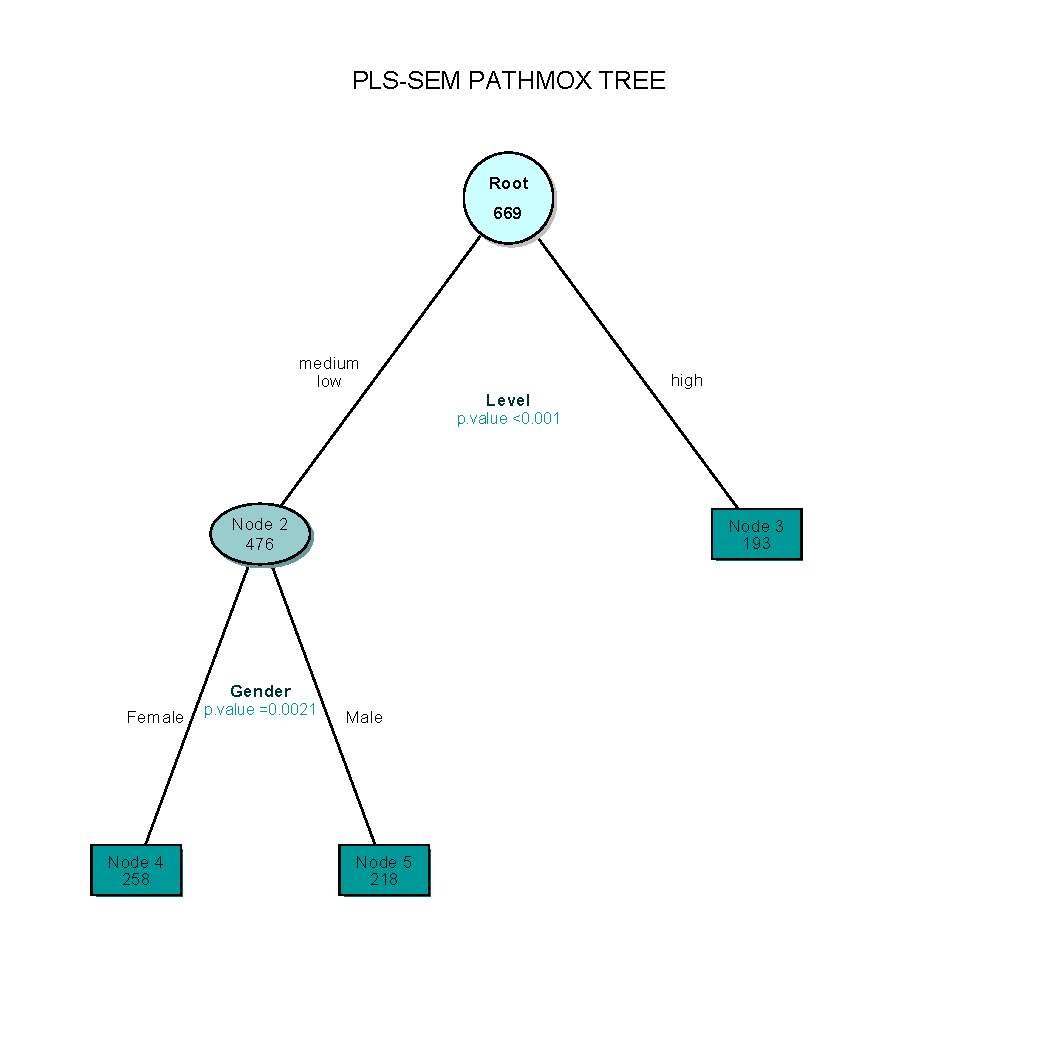
\includegraphics[width=0.6\textwidth]{Fig2_treeplot} &  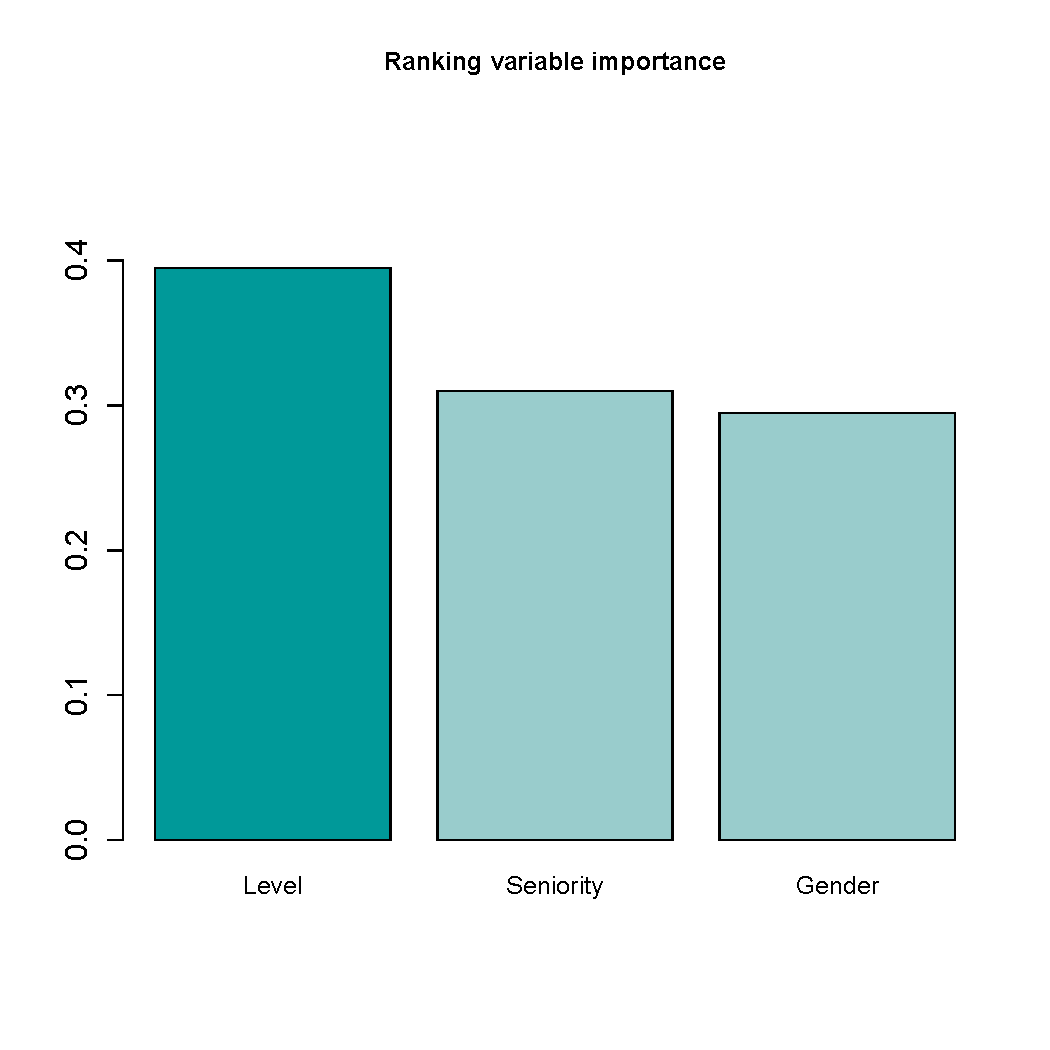
\includegraphics[width=0.4\textwidth]{FIg3_barimp}\\  \multicolumn{2}{c}{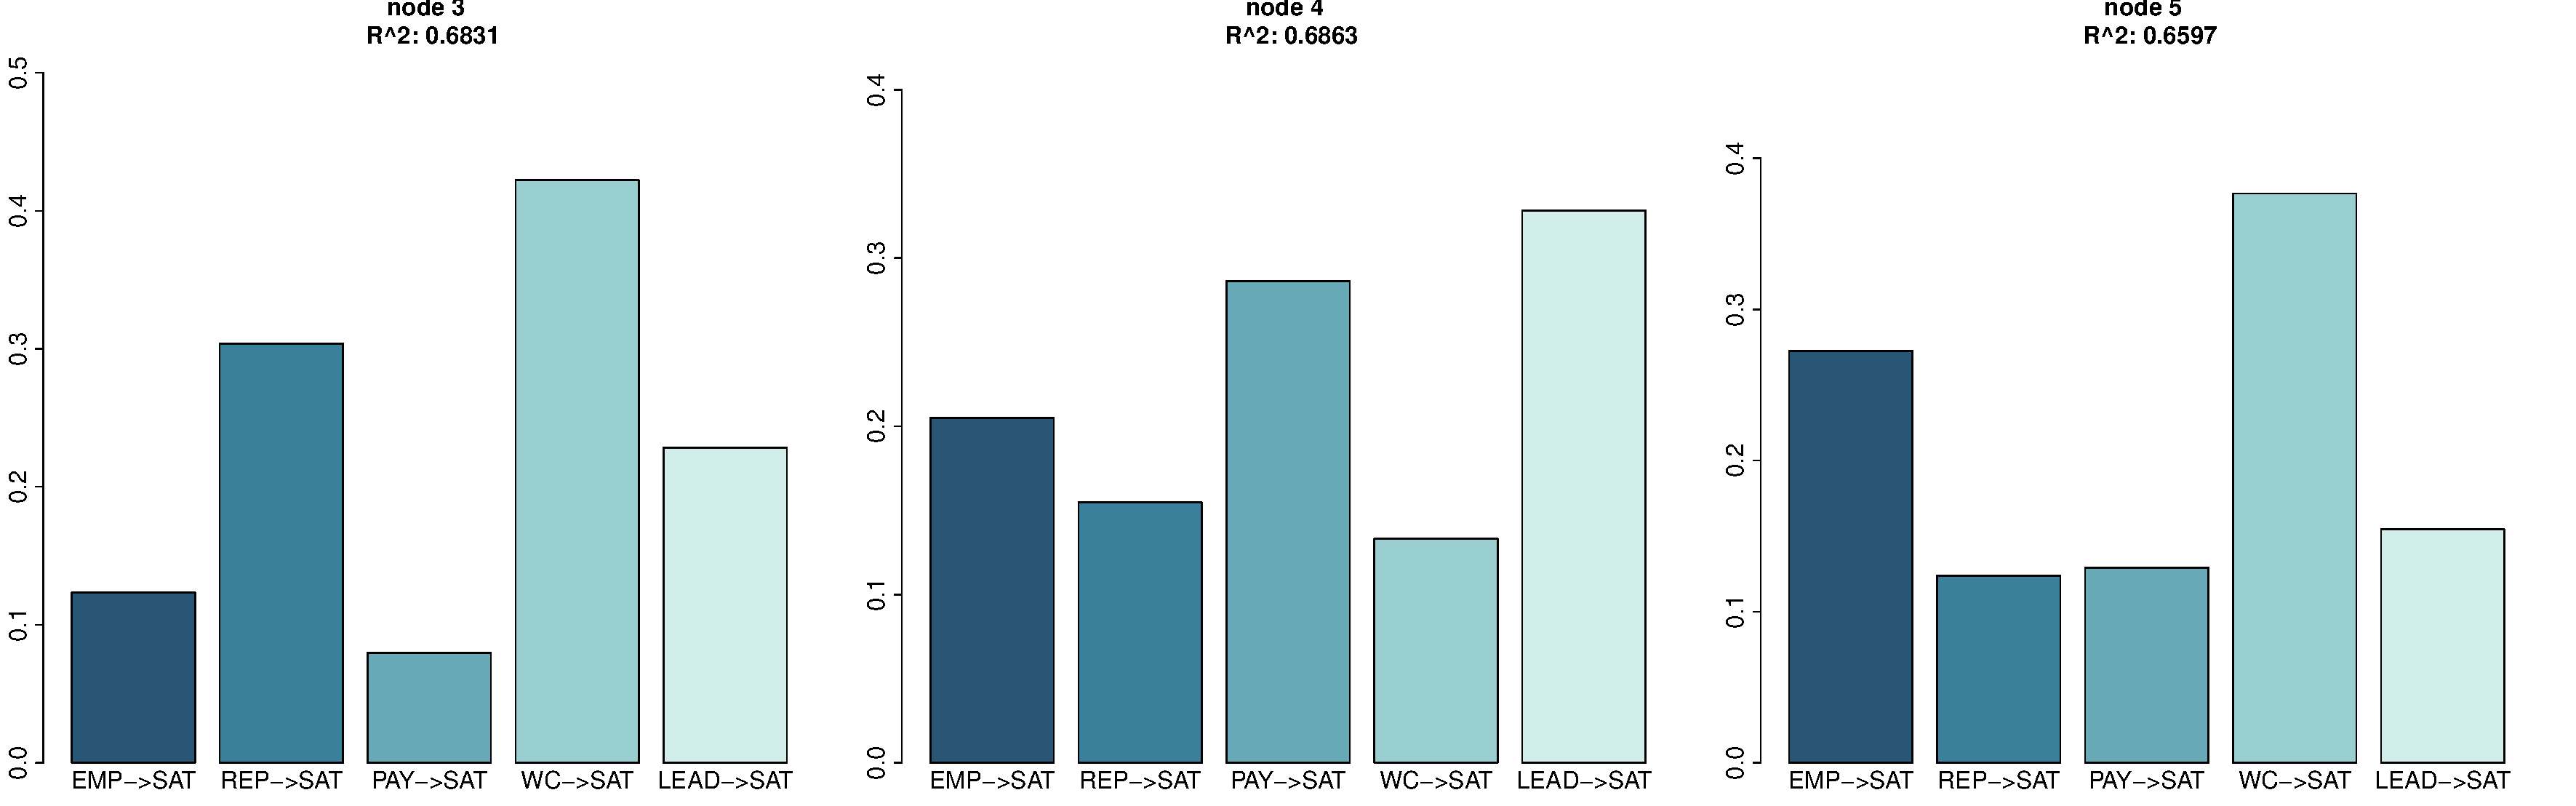
\includegraphics[width=1\textwidth]{Fig4_barcomp}} \end{array}\)

\hypertarget{terminal-node-outputs}{%
\subsection{Terminal node outputs}\label{terminal-node-outputs}}

Specific terminal nodes can be analyzed using the cSEM package function
csem(). By default the csem() function needs two parameters: the
datasets that include all indicators ( .data), and the PLS-SEM model
relationships ( .model). As we are interested in the results of the
terminal nodes, we pass the hybrid list in the " plstree" object to
the .data parameter, and use the same formula object defined for the
pls.pathmox() function. Below we reproduce the code, but not the output,
as not directly related with the genpathmox package.

\hypertarget{hybrid-multigroup-approach-lamberti21-invariance-and-multigroup-analysis}{%
\subsection{Hybrid multigroup approach (Lamberti 2021): invariance and multigroup analysis}\label{hybrid-multigroup-approach-lamberti21-invariance-and-multigroup-analysis}}

For the invariance and the multigroup comparison of the terminal nodes
identified by pathmox, we pass the object generated by the csem()
function to the testMICOM() and testMGD() functions. Note that, for the
multigroup comparison, we need to indicate which coefficients to compare
by fixing the parameter .parameters\_to\_compare. We generate the work
climate model, but this time only indicating the causal relationship
between the LVs. Finally, we indicate which statistical test to use for
comparison using the .approach\_mgd parameter (for our example, the
permutation test, .approach\_mgd = " Chin"). Below we reproduce the
code to show how genpathmox interfaces with cSEM, omitting the results
as there are not directly produced by the genpathmox package.

\begin{example}
\# MICOM procedure climateMICOM = testMICOM(terminal\_nodes\_results)

\# define the relationship between LVs climateMICOM =
testMICOM(terminal\_nodes\_results)

climate\_innermodel = " \# Structural model SAT ~ EMP + REP + PAY + WC +
LEAD LOY ~ SAT " \# multigroup analysis climateMGA =
testMGD(terminal\_nodes\_results, .parameters\_to\_compare =
climate\_innermodel, .approach\_mgd = "Chin")
\end{example}

\hypertarget{summary}{%
\section{Summary}\label{summary}}

The genpathmox \emph{R} package handles observed heterogeneity in PLS-SEM
models when the number of CVs is high and we do not know what the most
significant groupings could be. Development of genpathmox reflects the
statistical framework described in Lamberti (2021), and Lamberti, Banet Aluja, and Sanchez (2017; Lamberti, Aluja, and Sanchez 2016), and the package has several functions that enable
estimation and visualization of tree partitions. By using genpathmox,
users can quickly explore the effects of heterogeneity on their PLS-SEM
models and identify groups that may contribute to significant
differences.

\hypertarget{references}{%
\section*{References}\label{references}}
\addcontentsline{toc}{section}{References}

\hypertarget{refs}{}
\begin{CSLReferences}{1}{0}
\leavevmode\vadjust pre{\hypertarget{ref-Beker22}{}}%
Becker, Jan Michael, Jun Hwa Cheah, Rasoul Gholamzade, Christian M Ringle, and Marko Sarstedt. 2022. {``PLS-SEM's Most Wanted Guidance.''} \emph{International Journal of Contemporary Hospitality Management}. \url{https://doi.org/10.1108/IJCHM-04-2022-0474}.

\leavevmode\vadjust pre{\hypertarget{ref-Chin10}{}}%
Chin, Wynne W, and Jens Dibbern. 2010. {``An Introduction to a Permutation Based Procedure for Multi-Group PLS Analysis: Results of Tests of Differences on Simulated Data and a Cross Cultural Analysis of the Sourcing of Information System Services Between Germany and the USA.''} In \emph{Handbook of Partial Least Squares}, 171--93. Berlin Heidelberg: Springer. \url{https://doi.org/10.1007/978-3-540-32827-8_8}.

\leavevmode\vadjust pre{\hypertarget{ref-Chow60}{}}%
Chow, Gregory C. 1960. {``Tests of Equality Between Sets of Coefficients in Two Linear Regressions.''} \emph{Econometrica: Journal of the Econometric Society}, 591--605. \url{https://doi.org/10.2307/1910133}.

\leavevmode\vadjust pre{\hypertarget{ref-Dijkstra15}{}}%
Dijkstra, Theo K, and Jörg Henseler. 2015. {``Consistent Partial Least Squares Path Modeling.''} \emph{MIS Quarterly} 39 (2): 297--316. \url{https://www.jstor.org/stable/26628355}.

\leavevmode\vadjust pre{\hypertarget{ref-Vinzi08}{}}%
Esposito Vinzi, Vincenzo, Laura Trinchera, Silvia Squillacciotti, and Michel Tenenhaus. 2008. {``REBUS-PLS: A Response-Based Procedure for Detecting Unit Segments in PLS Path Modelling.''} \emph{Applied Stochastic Models in Business and Industry} 24 (5): 439--58. \url{https://doi.org/10.1002/asmb.728}.

\leavevmode\vadjust pre{\hypertarget{ref-Evermann21}{}}%
Evermann, Joerg, and Mikko Rönkkö. 2021. {``Recent Developments in PLS.''} \emph{Communications of the Association for Information Systems} 44: 123--32. \url{https://doi.org/10.17705/1CAIS.044XX}.

\leavevmode\vadjust pre{\hypertarget{ref-Hair21}{}}%
Hair Jr, Joseph F, G Tomas M Hult, Christian M Ringle, Marko Sarstedt, Nicholas P Danks, and Soumya Ray. 2021. \emph{Partial Least Squares Structural Equation Modeling (PLS-SEM) Using r: A Workbook}. Los Angeles: Springer Nature. \url{https://doi.org/10.1007/978-3-030-80519-7}.

\leavevmode\vadjust pre{\hypertarget{ref-Hair16}{}}%
Hair Jr, Joseph F, G. Tomas M. Hult, Christian Ringle, and Marko Sarstedt. 2016. \emph{A Primer on Partial Least Squares Structural Equation Modeling (PLS-SEM)}. Los Angeles: saGe publications. \url{https://doi.org/10.1007/978-3-030-80519-7}.

\leavevmode\vadjust pre{\hypertarget{ref-Hair17b}{}}%
Hair Jr, Joseph F, Lucy M Matthews, Ryan L Matthews, and Marko Sarstedt. 2017. {``PLS-SEM or CB-SEM: Updated Guidelines on Which Method to Use.''} \emph{International Journal of Multivariate Data Analysis} 1 (2): 107--23. \url{https://doi.org/10.1504/IJMDA.2017.087624}.

\leavevmode\vadjust pre{\hypertarget{ref-Hair19}{}}%
Hair Jr, Joseph F, Jeffrey J Risher, Marko Sarstedt, and Christian M. and Ringle. 2019. {``When to Use and How to Report the Results of PLS-SEM.''} \emph{European Business Review} 31 (1): 2--24. \url{https://doi.org/10.1108/EBR-11-2018-0203}.

\leavevmode\vadjust pre{\hypertarget{ref-Hair17}{}}%
Hair Jr, Joseph F, Marko Sarstedt, Christian M Ringle, and Siegfried P Gudergan. 2017. \emph{Advanced Issues in Partial Least Squares Structural Equation Modeling}. Los Angeles: saGe publications.

\leavevmode\vadjust pre{\hypertarget{ref-henseler21}{}}%
Henseler, Jörg. 2020. \emph{Composite-Based Structural Equation Modeling: Analyzing Latent and Emergent Variables}. New York: Guilford Publications.

\leavevmode\vadjust pre{\hypertarget{ref-Henseler16}{}}%
Henseler, Jörg, Christian M Ringle, and Marko Sarstedt. 2016. {``Testing Measurement Invariance of Composites Using Partial Least Squares.''} \emph{International Marketing Review} 3 (3): 405--31. \url{https://doi.org/10.1108/IMR-09-2014-0304}.

\leavevmode\vadjust pre{\hypertarget{ref-Henseler09}{}}%
Henseler, Jörg, Christian M Ringle, and Rudolf R Sinkovics. 2009. {``The Use of Partial Least Squares Path Modeling in International Marketing.''} In \emph{New Challenges to International Marketing}, 277--319. Bingley: Emerald Group Publishing Limited. \url{https://doi.org/10.1108/S1474-7979(2009)0000020014}.

\leavevmode\vadjust pre{\hypertarget{ref-Keil00}{}}%
Keil, Mark, Bernard CY Tan, Kwok Kee Wei, Timo Saarinen, Virpi Tuunainen, and Arjen Wassenaar. 2000. {``A Cross-Cultural Study on Escalation of Commitment Behavior in Software Projects.''} \emph{MIS Quarterly}, 299--325. \url{https://doi.org/10.2307/3250940}.

\leavevmode\vadjust pre{\hypertarget{ref-Klesel19}{}}%
Klesel, Michael, Florian Schuberth, Jörg Henseler, and Bjoern Niehaves. 2019. {``A Test for Multigroup Comparison Using Partial Least Squares Path Modeling.''} \emph{Internet Research} 29 (3): 464--77.\href{\%20https://doi.org/10.1108/IntR-11-2017-0418}{ https://doi.org/10.1108/IntR-11-2017-0418}.

\leavevmode\vadjust pre{\hypertarget{ref-Klesel22}{}}%
Klesel, Michael, Florian Schuberth, Björn Niehaves, and Jörg Henseler. 2022. {``Multigroup Analysis in Information Systems Research Using PLS-PM: A Systematic Investigation of Approaches.''} \emph{ACM SIGMIS Database: The DATABASE for Advances in Information Systems} 53 (3): 26--48. \url{https://doi.org/10.1145/3551783.3551787}.

\leavevmode\vadjust pre{\hypertarget{ref-Kollmann20}{}}%
Kollmann, Tobias, Christoph Stöckmann, Julia M Kensbock, and Anika Peschl. 2020. {``What Satisfies Younger Versus Older Employees, and Why? An Aging Perspective on Equity Theory to Explain Interactive Effects of Employee Age, Monetary Rewards, and Task Contributions on Job Satisfaction.''} \emph{Human Resource Management} 59 (1): 101--15. \url{https://doi.org/10.1002/hrm.21981}.

\leavevmode\vadjust pre{\hypertarget{ref-Lamberti21}{}}%
Lamberti, Giuseppe. 2021. {``Hybrid Multigroup Partial Least Squares Structural Equation Modelling: An Application to Bank Employee Satisfaction and Loyalty.''} \emph{Quality \(\&\) Quantity}, 1--23. \url{https://doi.org/10.1007/s11135-021-01096-9}.

\leavevmode\vadjust pre{\hypertarget{ref-genpathmox}{}}%
---------. 2022. \emph{Genpathmox: Pathmox Approach Segmentation Tree Analysis}. \url{https://CRAN.R-project.org/package=genpathmox}.

\leavevmode\vadjust pre{\hypertarget{ref-Lamberti20}{}}%
Lamberti, Giuseppe, Tomas Aluja Banet, and Josep Rialp Criado. 2020. {``Work Climate Drivers and Employee Heterogeneity.''} \emph{The International Journal of Human Resource Management} 33 (3): 472--504. \url{https://doi.org/10.1080/09585192.2020.1711798}.

\leavevmode\vadjust pre{\hypertarget{ref-Lamberti16}{}}%
Lamberti, Giuseppe, Tomas Banet Aluja, and Gaston Sanchez. 2016. {``The Pathmox Approach for PLS Path Modeling Segmentation.''} \emph{Applied Stochastic Models in Business and Industry} 32 (4): 453--68. \url{https://doi.org/10.1002/asmb.2168}.

\leavevmode\vadjust pre{\hypertarget{ref-Lamberti17}{}}%
Lamberti, Giuseppe, Tomas Banet Aluja, and Gaston Sanchez. 2017. {``The Pathmox Approach for PLS Path Modeling: Discovering Which Constructs Differentiate Segments.''} \emph{Applied Stochastic Models in Business and Industry} 33 (6): 674--89. \url{https://doi.org/10.1002/asmb.2270}.

\leavevmode\vadjust pre{\hypertarget{ref-Lebart79}{}}%
Lebart, Ludovic, Alain Morineau, and Jean Pierre Fenelon. 1979. \emph{Traitement Des Donnees Statistiques}. Paris: Dunod.

\leavevmode\vadjust pre{\hypertarget{ref-loh97}{}}%
Loh, Wei Yin, and Yu Shan Shih. 1997. {``Split Selection Methods for Classification Trees.''} \emph{Statistica Sinica}, 815--40. \url{https://www.jstor.org/stable/24306157}.

\leavevmode\vadjust pre{\hypertarget{ref-csem}{}}%
Rademaker, Manuel E., and Florian Schuberth. 2020. \emph{cSEM: Composite-Based Structural Equation Modeling}. \url{https://CRAN.R-project.org/package=cSEM}.

\leavevmode\vadjust pre{\hypertarget{ref-seminr}{}}%
Ray, Soumya, Nicholas P. Danks, and Andre C. Valdez. 2020. \emph{Seminr: Building and Estimating Structural Equation Models}. \url{https://CRAN.R-project.org/package=seminr}.

\leavevmode\vadjust pre{\hypertarget{ref-matpls}{}}%
Rönkkö, Mikko. 2017. \emph{Matrixpls: Matrix-Based Partial Least Squares Estimation}. \url{https://github.com/mronkko/matrixpls}.

\leavevmode\vadjust pre{\hypertarget{ref-lavaan}{}}%
Rosseel, Yves. 2012. {``Lavaan: An r Package for Structural Equation Modeling.''} \emph{Journal of Statistical Software} 48 (2): 1--36. \url{https://doi.org/10.18637/jss.v048.i02}.

\leavevmode\vadjust pre{\hypertarget{ref-Sanchez06}{}}%
Sanchez, Gaston, and Tomas Aluja. 2006. {``Pathmox: A PLS-PM Segmentation Algorithm.''} \emph{Proceedings of KNEMO} 69.

\leavevmode\vadjust pre{\hypertarget{ref-plspm}{}}%
Sanchez, Gaston, Laura Trinchera, and Giorgio Russolillo. 2015. \emph{Plspm: Tools for Partial Least Squares Path Modeling (PLS-PM)}. \url{https://github.com/gastonstat/plspm}.

\leavevmode\vadjust pre{\hypertarget{ref-Sarstedt22a}{}}%
Sarstedt, Marko, Joseph F Hair, Mandy Pick, Benjamin D Liengaard, Lăcrămioara Radomir, and Christian M Ringle. 2022. {``Progress in Partial Least Squares Structural Equation Modeling Use in Marketing Research in the Last Decade.''} \emph{Psychology \(\&\) Marketing} 39 (5): 1035--64.\href{\%20https://doi.org/10.1002/mar.21640}{ https://doi.org/10.1002/mar.21640}.

\leavevmode\vadjust pre{\hypertarget{ref-Sarstedt22b}{}}%
Sarstedt, Marko, Joseph F Hair Jr, and Christian M Ringle. 2022. {``PLS-SEM: Indeed a Silver Bullet--Retrospective Observations and Recent Advances.''} \emph{Journal of Marketing Theory and Practice}, 1--15. \url{https://doi.org/10.1080/10696679.2022.2056488}.

\leavevmode\vadjust pre{\hypertarget{ref-Sarstedt22c}{}}%
Sarstedt, Marko, Lăcrămioara Radomir, Ovidiu Ioan Moisescu, and Christian M Ringle. 2022. {``Latent Class Analysis in PLS-SEM: A Review and Recommendations for Future Applications.''} \emph{Journal of Business Research} 138: 398--407. \url{https://doi.org/10.1016/j.jbusres.2021.08.051}.

\leavevmode\vadjust pre{\hypertarget{ref-Shmueli16}{}}%
Shmueli, Galit, Soumya Ray, Juan Manuel Velasquez Estrada, and Suneel Babu Chatla. 2016. {``The Elephant in the Room: Predictive Performance of PLS Models.''} \emph{Journal of Business Research} 69 (10): 4552--64. \url{https://doi.org/10.1016/j.jbusres.2016.03.049}.

\leavevmode\vadjust pre{\hypertarget{ref-Shmueli19}{}}%
Shmueli, Galit, Marko Sarstedt, Joseph F Hair, Jun Hwa Cheah, Hiram Ting, Santha Vaithilingam, and Christian M Ringle. 2019. {``Predictive Model Assessment in PLS-SEM: Guidelines for Using PLSpredict.''} \emph{European Journal of Marketing} 53 (11): 2322--47. \url{https://doi.org/10.1108/EJM-02-2019-0189}.

\leavevmode\vadjust pre{\hypertarget{ref-diagram}{}}%
Soetaert, Karline. 2020. \emph{Diagram: Functions for Visualising Simple Graphs (Networks), Plotting Flow Diagrams}. \url{https://CRAN.R-project.org/package=diagram}.

\leavevmode\vadjust pre{\hypertarget{ref-Wold85}{}}%
Wold, Herman. 1985. {``Partial Least Squares.''} In \emph{Encyclopedia of Statistical Sciences}, 6:581--91. John Wiley; Sons, Ltd. \url{https://doi.org/10.1002/0471667196.ess1914.pub2}.

\end{CSLReferences}


\address{%
Giuseppe Lamberti,\\
Department of Business,\\%
Universitat Autonoma de Barcelona UAB,\\ Spain.\\ \url{http://orcid.org/0000-0002-8666-796X}\\
%
%
%
\href{mailto:giuseppe.lamberti@uab.cat}{\nolinkurl{giuseppe.lamberti@uab.cat}}%
}

\end{article}


\end{document}
